% 2016
% Maciej Szeptuch
% II UWr

\documentclass[polish, t,10pt]{beamer}
\usetheme{Antibes}
\usecolortheme{lily}
\setbeamertemplate{footline}[frame number]
\setbeamertemplate{navigation symbols}{}

\usepackage[utf8]{inputenc}
\usepackage{polski}
\usepackage{babel}

\usepackage{multicol}
\usepackage{graphicx}
\usepackage{wrapfig}

%% Kropka po numerze paragrafu, podparagrafu, itp.
\makeatletter
    \renewcommand\@seccntformat[1]{\csname the#1\endcsname.\quad}
    \renewcommand\numberline[1]{#1.\hskip0.7em}
\makeatother

%% Numeracja wzorów
\renewcommand{\theequation}{\arabic{section}.\arabic{equation}}

%% Plan przed każdą sekcją
\AtBeginSection[]
{
    \begin{frame}<beamer>
        \tableofcontents[currentsection]
    \end{frame}
}

%%%%%%%%%%%%%%%%%%%%%%%%%%%%%%%%%%%%%%%%%%%%%%%%%%%%%%%%%%%%%%%%%%%%%%%%%%%%%%%

\title{Modelowanie interferencji w sieciach bezprzewodowych}
\subtitle{SINR a Grafy Konfliktu}
\author{Maciej Szeptuch}
\date{Wrocław, \today}

\begin{document}

% STRONA TYTUŁOWA
\begin{frame}
    \titlepage
\end{frame}

% PLAN
\begin{frame}
    \frametitle{Plan}
    \tableofcontents
\end{frame}

\def \si {{\color{green}s_i}}
\def \sj {{\color{green}s_j}}
\def \sno {{\color{green}s_{n+1}}}
\def \snt {{\color{green}s_{n+2}}}

\def \ri {{\color{red}r_i}}
\def \rj {{\color{red}r_j}}
\def \rrj {{\color{red}j}}
\def \rno {{\color{red}r_{n+1}}}
\def \rnt {{\color{red}r_{n+2}}}

\def \Li {{\color{blue}L_i}}
\def \li {{\color{blue}l_i}}
\def \Lj {{\color{blue}L_j}}
\def \lj {{\color{blue}l_j}}
\def \Lo {{\color{blue}L_1}}
\def \Ln {{\color{blue}L_n}}
\def \Lno {{\color{blue}L_{n+1}}}
\def \Lnt {{\color{blue}L_{n+2}}}
\def \Lm {{\color{blue}L_m}}

\def \dii {{\color{cyan}d_{i.i}}}
\def \dij {{\color{cyan}d_{i.j}}}
\def \dji {{\color{cyan}d_{j.i}}}
\def \djj {{\color{cyan}d_{j.j}}}

% Opis
\section{SINR}
\subsection{Model}
    \begin{frame}
        \frametitle{Model}
        Oznaczenia:
        \begin{itemize}
            \item $\mathcal{L} = \{\Lo, \ldots, \Ln\}$ - zbiór połączeń
            \item $\Li = (\si, \ri)$ $\li = |\Li| = \dii$ - jedno połączenie, jego długość
            \item $\dij = d(\si, \rj)$ - odległość między nadajnikiem a odbiornikiem
            \item $\Delta(\mathcal{L}) = \frac{\max{|\Li|}}{\min{|\Li|}}$ - stosunek maksymalnej do minimalnej długości połączenia
            \item $d(i,j) = \min(\dij, \dji, d(\si, \sj), d(\ri, \rj))$ - odległość pomiędzy połączeniami
        \end{itemize}
    \end{frame}
    \begin{frame}
        \frametitle{Model}
        Oznaczenia cd.:
        \begin{itemize}
            \item $P(\si)$ - moc
            \item $\dij^{-\alpha}$ - strata sygnału
            \item $\alpha$ - zazwyczaj $2 \le \alpha \leq 6$
            \item $P_{ii} = P_{\ri}(\si) = P(\si) \cdot \li^{-\alpha}$ - moc odbierana
            \item $I_{ji} = I_{\rj}(\si) = P_{\rj}(\si)$ - interferencja jednego połączenia
            \item $I_{\ri} = I_{\ri}(\mathcal{L}) = \sum_{\Lj \in \mathcal{L}, \Lj \neq \Li} I_{\ri}(\sj)$ - interferencja na odbiorniku
        \end{itemize}
    \end{frame}
    \begin{frame}
        Oznaczenia cd.:
        \begin{itemize}
            \item $N$ - szum otoczenia
            \item $SINR_{\Li} = SINR_{\Li}(\mathcal{L}) = \frac{P_{\ri}(\si)}{I_{\ri} + N}$ - współczynnik sygnału do szumu i interferencji
            \item $\beta$ - współczynnik odbioru sygnału, zależny od sprzętu
            \item sygnał na danym połączeniu jest poprawnie odbierany wtw. $SINR_{\Li} \geq \beta$
            \item harmonogram $\mathcal{S} = \{\mathcal{S}_1, \ldots, \mathcal{S}_T\}$ jest wykonalny jeśli $\forall_{\mathcal{S}_t \in \mathcal{S}} \forall_{\Li \in \mathcal{S}_t} SINR_{\Li}(\mathcal{S}_t) \geq \beta$
        \end{itemize}
    \end{frame}

\subsection{Problemy}
    \begin{frame}
        \frametitle{Problemy}
        \begin{wrapfigure}{R}{0.5\textwidth}
            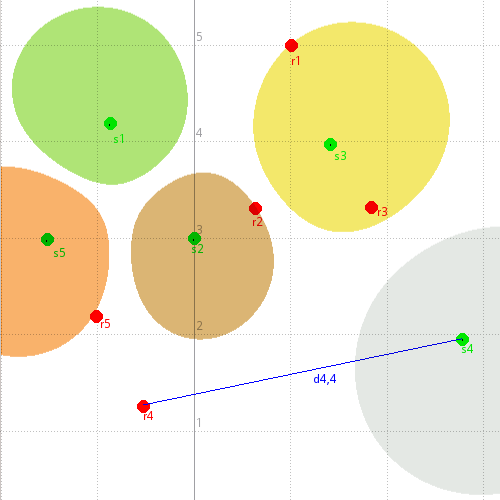
\includegraphics[width=0.5\textwidth]{pictures/model.png}
            \caption{Przykładowa wizualizacja modelu}
        \end{wrapfigure}
        Najważniejsze problemy:
        \begin{itemize}
            \item (Weighted) One-Slot - jak najwięcej połączeń na raz
            \item Multi-Slot - jak najmniej przedziałów
        \end{itemize}
    \end{frame}

\section{Graf Konfliktu (Conflict Graph)}
\subsection{Model}
    \begin{frame}
        Chcemy reprezentować to samo co SINR (prawie) ale za pomocą grafów. \\
        Jak taki graf miałby wyglądać? \\
        \pause
        Wierzchołkami będą połączenia, a krawędzie będą oznaczać, że dane dwa połączenia nie są jednocześnie wykonalne. \\
        \pause
        Reguły (aksjomaty) tworzenia grafu na podstawie zbioru połączeń: \\
        \begin{block}{Aksjomat 1}
            Schemat tworzenia grafu konfliktu jest zdefiniowany przez wzajemne relacje na połączeniach.
        \end{block}

        \pause
        \begin{block}{Aksjomat 2}
            Schemat tworzenia grafu konfliktu jest niezależny od pozycji i skali.
        \end{block}

        \pause
        \begin{block}{Aksjomat 3}
            Schemat jest monotoniczny wraz ze wzrostem odległości.
        \end{block}

        \pause
        \begin{block}{Aksjomat 4}
            Jeżeli dwa połączenia nie mogą istnieć w jednym rozwiązaniu muszą być połączone krawędzią w grafie konfliktu.
        \end{block}
    \end{frame}
    \begin{frame}
        \begin{block}{Aksjomat 5}
            W przypadku możliwości dowolnej regulacji mocy, schemat jest symetryczny ze względu na nadajniki i odbiorniki.
        \end{block}
        \pause
        ~\\
        \begin{definition}
            Niech $f$ będzie dodatnią, niemalejącą podliniową funkcją. Dwa połączenia $i,j$ nazwiemy \textit{f-niezależnymi} jeśli
            $$
            \frac{d(i,j)}{l_{min}} > f(\frac{l_{max}}{l_{min}})
            $$
            gdzie $l_{min} = \min(\li,\lj)$, $l_{max} = \max(\li,\lj)$ i w przeciwnym wypadku są \textit{f-sąsiadujące}. \\
            Zbiór połączeń jest \textit{f-niezależny}(\textit{f-sąsiadujący}) jeśli połączenia są parami \textit{f-niezależne}(\textit{f-sąsiadujące}). \\
            Niech $\mathcal{L}$ będzie zbiorem połączeń. Graf konfliktu $\mathcal{G}_f(\mathcal{L})$ to graf z wierzchołkami $\mathcal{L}$, które są połączone wtw. gdy są \textit{f-sąsiadujące}.
        \end{definition}
    \end{frame}
    \begin{frame}
        \begin{theorem}[1]
            Dla dowolnej stałej $\gamma > 0$ \textit{$(\gamma + 1)^{\alpha}$-wykonalny} zbiór jest \textit{$\gamma$-niezależny}.
        \end{theorem}
        gdzie zbiór jest \textit{$\gamma$-wykonalny} jeśli jest wykonalny przy zamianie parametru $\beta$ na $\gamma$. \\
        \begin{proof}
            Szkic. \\
            \begin{itemize}
                \item Wystarczy pokazać że dwa połączenia w tym samym \textit{$(\gamma + 1)^{\alpha}$-wykonalnym} zbiorze muszą być \textit{$\gamma$-niezależne}
                \item Istnieje odpowiedni przydział mocy $P(i)/l_i^{\alpha} > (\gamma + 1)^{\alpha}P(j)/d_{ji}^{\alpha}$
                \item Przemnażamy, otrzymując $d_{ij}d_{ji} > (\gamma + 1)^2l_i l_j$
                \item Nie wprost i nierówności trójkąta
                \item w końcu dochodzimy do $d(i,j) > \gamma\min(l_i,l_j)$
            \end{itemize}
        \end{proof}
    \end{frame}
    \begin{frame}
        \begin{block}{Wniosek}
            Każdy schemat tworzenia grafu konfliktu spełniający powyższe aksjomaty jest zasadniczo postaci $\mathcal{G}_f$, dla pewnej funkcji $f$. Może się różnić od $\mathcal{G}_f$ co najwyżej odpowiednią stałą.
        \end{block}

        \begin{block}{Dowód.}
            Pokażemy że dowolny schemat tworzenia grafu konfliktu $\mathcal{K}$ zawiera się pomiędzy $\mathcal{G}_f$ a $\mathcal{G}_{\gamma f}$, tj. $\mathcal{G}_f(\mathcal{L}) \subseteq \mathcal{K}(\mathcal{L}) \subseteq \mathcal{G}_{\gamma f}(\mathcal{L})$. \\
            Szkic: \\
            \begin{itemize}
                \item Chcemy pokazać że decyzja o istnieniu krawędzi między połączeniami może zostać podjęta tylko na podstawie najkrótszej odległości wśród 4 punktów tych połączeń oraz długości dłuższego z nich
                \item $\mathcal{K}$ musi spełniać aksjomaty
                \item Z Aksjomatu 1 $\mathcal{K}$ jest funkcją nad parami połączeń, konkretniej odległościami w nich
                \item Z Aksjomatu 2 możemy normalizować odległości używając długości krótszego połączenia
            \end{itemize}
        \end{block}
    \end{frame}
    \begin{frame}
        \begin{itemize}
            \item Z Aksjomatu 5 nie ma znaczenia kto nadaje a kto odbiera
            \item Z Aksjomatu 4 niekompatybilne połączenia muszą być połączone krawędzią w każdym grafie konfliktu więc możemy spojrzeć tylko na te jednocześnie wykonalne
            \item Korzystając z Twierdzenia 1 mamy ograniczenie z dołu na odległość pomiędzy połączeniami zależną od długości krótszego połączenia
            \item Stosujemy parę razy nierówność trójkąta co pozwala nam ograniczyć pozostałe odległości
            \item Korzystając z Aksjomatu 3 (monotoniczności) mamy że $\mathcal{K}$ można zdefiniować przez monotoniczny predykat dwóch zmiennych odległości pomiędzy połączeniami oraz długości dłuższego z nich
            \item Ale dowolny monotoniczny predykat zmiennych $x,y$ można reprezentować jako relację postaci $y > f(x)$ dla pewnej $f$.
        \end{itemize}
    \end{frame}

\subsection{Własności}
\subsubsection{Różnica między liczbą chromatyczną grafów konfliktu}
    \begin{frame}
        \frametitle{Liczba chromatyczna w grafie konfliktu}
        \begin{theorem}
            Dla dowolnego zbioru połączeń $\mathcal{L}$, stałej $\gamma \ge 1$ oraz niemalejącej, silnie podliniowej funkcji $f$
            $\chi(\mathcal{G}_{\gamma f}(\mathcal{L})) = O(f^{*}(\Delta)) \cdot \chi(\mathcal{G}_{\gamma}(\mathcal{L}))$.
        \end{theorem}
        \begin{proof}
            Szkic.
            \begin{itemize}
                \item Niech S będzie \textit{$\gamma$-niezależnym} podzbiorem $\mathcal{L}$.
                \item Popatrzymy na dowolne połączenie $i$ oraz zbiór $T$ reprezentujący połączenia w $S^{+}_i$ które są \textit{$f$-sąsiadujące} z $i$
                \item Pokażemy że $T = O(log^{*}(\Delta))$
                \item Niech $p_j$ będzie końcem połączenia $j \in T$ najbliższym do $i$.
                \item Podzielimy T na dwie części względem odległości do końców połączenia $i$ i zajmiemy się jedną z nich
                \item Nierówność trójkąta
                \item Kolejny podział na dwie części
                \item Własność podwajania (doubling property) oraz funkcja iterowana
            \end{itemize}
        \end{proof}
    \end{frame}
    \begin{frame}
        \begin{theorem}
            Dla dowolnego zbioru połączeń $\mathcal{L}$, stałej $\gamma > 0$ oraz niemalejącej, silnie podliniowej funkcji $f$
            $\chi(\mathcal{G}_f(\mathcal{L})) = \Theta(\chi(\mathcal{G}_{\gamma f}(\mathcal{L})))$.
        \end{theorem}
        \begin{lemma}[1]
            Niech $f$ będzie niemalejącą, silnie podliniową funkcją a $i,j,k$ będą połączeniami. Jeśli $j,k$ są dłuższe niż $i$, są \textit{$f$-niezależne} oraz są \textit{$\gamma f$-siąsadujące} z $i$ wtedy $\min (l_j,l_k) \le cl_i$, gdzie $c$ zależy tylko od $f$ oraz $\gamma$.
        \end{lemma}
        \begin{proof}
            Szkic.
            \begin{itemize}
                \item Podobnie jak wcześniej ustalamy $S$ oraz $i$
                \item Korzystamy z lematu żeby ograniczyć długość połączeń
                \item Podzielimy T na dwie części względem odległości do końców połączenia $i$ i zajmiemy się jedną z nich
                \item Korzystamy z \textit{$f$-niezależności} i własności podwajania
            \end{itemize}
        \end{proof}
    \end{frame}

\subsubsection{Aproksymowalność w grafach konfliktu}
    \begin{frame}
        \frametitle{Aproksymowalność w grafach konfliktu}
        \begin{theorem}
            Niech $f$ będzie funkcją t.że $f(x)/x$ jest nierosnące, oraz $\mathcal{L}$ będzie zbiorem połączeń na płaszczyźnie. Wtedy $\mathcal{G}_f(\mathcal{L})$ jest \textit{12-symplicjalny}.
        \end{theorem}
        \begin{proof}
            Szkic. \\
            \begin{itemize}
                \item Weźmy dowolne połączenie $i$
                \item Niech $S \subseteq L_i^{+}$ będzie zbiorem dłuższych sąsiadów $i$ w $\mathcal{G}_f(\mathcal{L})$
                \item Dzielimy $S$ na dwa zbiory: bliższych do nadajnika i bliższych do odbiornika
                \item Rozpatrzmy jeden z nich, podzielmy płaszczyznę na 6 równych części
                \item Popatrzmy na połączenia znajdujące się w jednej z nich
                \item Muszą być sąsiadami
                \item Wystarczy 6 klik żeby je pokryć
                \item Analogicznie dla drugiego zbioru
            \end{itemize}
        \end{proof}
    \end{frame}
    \begin{frame}
        \begin{theorem}
            Niech $f$ będzie niemalejącą, silnie podliniową funkcją z $f(x) \ge 1$ dla $x \ge 1$. Wtedy dla dowolnego zbioru połączeń $\mathcal{L}$ $\mathcal{G}_f(\mathcal{L})$ jest \textit{stało-symplicjalny}.
        \end{theorem}
        \begin{proof}
            Szkic.
            \begin{itemize}
                \item Podobnie patrzymy na $i$ oraz $S \subseteq L_i^{+}$
                \item Korzystając z Lematu 1 połączenia dłuższe niż $cl_i$ tworzą klikę
                \item Pozostałe sprytnie dzielimy
                \item Korzystając z nierówności trójkąta i własności podwajania można pokazać że powstanie stała liczba klik w poprzednim kroku
            \end{itemize}
        \end{proof}
    \end{frame}

\section{Aproksymacja SINR w Grafach Konfliktu}
\subsection{Niezależność wykonalnych zbiorów}
    \begin{frame}
        \frametitle{Niezależność wykonalnych zbiorów}
        \begin{theorem}[1]
            Dla dowolnej stałej $\gamma > 0$ \textit{$(\gamma + 1)^{\alpha}$-wykonalny} zbiór jest \textit{$\gamma$-niezależny}.
        \end{theorem}
        gdzie zbiór jest \textit{$\gamma$-wykonalny} jeśli jest wykonalny przy zamianie parametru $\beta$ na $\gamma$. \\
        \begin{proof}
            Szkic. \\
            \begin{itemize}
                \item Wystarczy pokazać że dwa połączenia w tym samym \textit{$(\gamma + 1)^{\alpha}$-wykonalnym} zbiorze muszą być \textit{$\gamma$-niezależne}
                \item Istnieje odpowiedni przydział mocy $P(i)/l_i^{\alpha} > (\gamma + 1)^{\alpha}P(j)/d_{ji}^{\alpha}$
                \item Przemnażamy, otrzymując $d_{ij}d_{ji} > (\gamma + 1)^2l_i l_j$
                \item Nie wprost i nierówności trójkąta
                \item w końcu dochodzimy do $d(i,j) > \gamma\min(l_i,l_j)$
            \end{itemize}
        \end{proof}
    \end{frame}

\subsection{Wykonalność niezależnych zbiorów}
    \begin{frame}
        \frametitle{Wykonalność niezależnych zbiorów}
        Pokażemy że wykonalność SINR zawiera się pomiędzy $\mathcal{G}_{\gamma}$ a $\mathcal{G}_f$ dla odpowiednich $\gamma$ oraz $f$.
        \begin{block}{Operator wpływu}
            \begin{itemize}
                \item dla połączeń $i,j$ Niech $I(i,j) = \frac{l_i^{\alpha}}{d(i,j)^{\alpha}}$
                \item dla uproszczenia niech $I(i,i) = 0$
                \item $I(S,i) = \sum_{j \in S} I(j,i)$ oraz $I(i,S) = \sum_{j \in S} I(i,j)$
                \item $I(\mathcal{L}) = \max_{i \in \mathcal{L}} I(L_i^{-},i)$
            \end{itemize}
        \end{block}
        \begin{theorem}{Wystarczający warunek wykonalności \\~\\}
            Dla dowolnego zbioru połączeń $\mathcal{L}$ w przestrzeni metrycznej jeśli $I(\mathcal{L}) < \frac{1}{2\cdot3^{\alpha} (4\beta+2)}$ wtedy $\mathcal{L}$ jest wykonalny.
        \end{theorem}
    \end{frame}
    \begin{frame}
        \frametitle{Wykonalność niezależnych zbiorów}
        Niech $\widehat{\log}(x) = \max(\log^{2/(\alpha-m)}(x),1)$. Pokażemy że dla dostatecznie dużej stałej $\gamma$, \textit{$\gamma\widehat{\log}$-niezależność} implikuje wykonalność. W szczególności pokażemy że jeśli zbiór $S$ jest \textit{$\gamma\widehat{\log}$-niezależny} wtedy $I(S) = O(\gamma^{m-\alpha})$. \\
        Argument składa się z następujących etapów. \\
        Najpierw dla dowolnego połączenia $i \in S$ dzielimy $S_i^{-}$ na klasy podobnej długości, gdzie podobna długość znaczy że połączenia w danym podzbiorze różnią się długością co najwyżej dwukrotnie. Ograniczymy wpływ na połączenie $i$ w każdym podzbiorze z osobna i następnie połączymy je korzystając z addytywności operatora $I$. \\
        Dla każdego z podzbiorów stosujemy podobną metodę: dzielimy przestrzeń na pierścienie wkoło $i$, zliczamy połączenia w każdym z pierścieni i ograniczamy $I(S_i^{-},i)$ bazując na nich oraz fakcie że mają podobny wpływ na $i$(są w mniej więcej tej samej odległości). \\
        Wpływ każdego podzbioru wychodzi $O((\gamma\widehat{\log}(l_i/l))^{m-\alpha}$. $\widehat{\log}$ został tak dobrany aby suma się zgodziła.
    \end{frame}

\section{Wnioski}
\subsection{Aproksymacja Multi-Slota i Ważonego One-Slota}
    \begin{frame}
        \frametitle{Aproksymacja Multi-Slota i Ważonego One-Slota}
        \begin{theorem}
            Istnieje $O(log^{*}(\Delta))$-aproksymacja dla multi-slota. Otrzymujemy ją poprzez pokolorowanie grafu $\mathcal{G}_{\gamma \widehat{log}}(\mathcal{L})$ (dla odpowiedniej stałej $\gamma$).
        \end{theorem}
        \begin{theorem}
            Istnieje $O(log^{*}(\Delta))$-aproksymacja dla ważonego one-slota. Otrzymujemy ją poprzez aproksymacje maksymalnego ważonego zbioru niezależnego grafu $\mathcal{G}_{\gamma \widehat{log}(\mathcal{L})}$ (dla odpowiedniej stałej $\gamma$).
        \end{theorem}
    \end{frame}

\section{Ograniczenia podejścia grafowego}
    \begin{frame}
        \frametitle{Ograniczenia podejścia grafowego}
        \begin{itemize}
            \item Nie istnieją żadne nietrywialne aproksymacje Multi-Slota ze względu na liczbę połączeń w tym modelu
            \item Pokazana aproksymacja jest najlepszą możliwą w tym modelu
            \item W metrykach bez własności podwajania ta metoda nie daje żadnych nietrywialnych aproksymacji
        \end{itemize}
    \end{frame}

\end{document}
